
%(BEGIN_QUESTION)
% Copyright 2010, Tony R. Kuphaldt, released under the Creative Commons Attribution License (v 1.0)
% This means you may do almost anything with this work of mine, so long as you give me proper credit

This PLC math instruction performs a calculation on four different 16-bit signed integers (decimal range = $-32768$ to +32767) {\tt N7:1} through {\tt N7:4}, storing the result of the expression in memory location {\tt N7:24}.  The expression shown in the CMP instruction box is evaluated according to standard mathematical order of operations, with each and every step of the calculation handled as a 16-bit signed integer number:

$$\includegraphics[width=15.5cm]{i02458x01.eps}$$

The live values of these 16-bit integers are shown here:

\begin{itemize}
\item{} {\tt N7:1} = 500
\item{} {\tt N7:2} = 15000
\item{} {\tt N7:3} = 750
\item{} {\tt N7:4} = 200
\end{itemize}

The PLC's evaluation of this expression will be flawed due to the limitations of signed 16-bit integer values.  First, identify where in the order of operations the calculation goes wrong, and then re-write the expression so that the PLC can successfully perform the calculation on these same values.  Note that your new expression must work with all the original values listed above ({\tt N7:1} through {\tt N7:4}).

\vskip 100pt

\underbar{file i02458}
%(END_QUESTION)





%(BEGIN_ANSWER)

500 $\times$ 15000 yields a value of 7.5 million, which exceeds the range of a signed 16-bit value (+32767 to - 32768).  The following re-write will work:

\vskip 10pt

{\tt ((N7:2 / N7:3 * N7:1) - N7:4)} 

\vskip 10pt

Performing the division of 15000 and 750 {\it before} multiplying by 500 solves the problem.

%(END_ANSWER)





%(BEGIN_NOTES)

{\bf This question is intended for exams only and not worksheets!}.

%(END_NOTES)

